\section{Conext-free grammar}

The linguist Chompsky sparked a revolution in the study of language by 
detailing grammar in a mathematical context.  To make a grammar
there is one forgoing assumption that we can take an alphabet of 
fixed symbols, traditionally denoted $\Sigma$, and from that 
have some concept of words over that alphabet.  For example 
$\Sigma\defeq\{a,b\}$ would mean that $aabaaabb$ is a string
of type $\Sigma^*$, the $*$ is known as the \emph{Kleene star},\index{Kleene star}.  We write $aabaaabb:\Sigma^*$.  For convenience we 
let $\epsilon$ denote the empty string.  More on this in a moment.

\subsection{Serializing}
Chompsky had and advantage that written human languages are largely serial
in that the character, words, and sentences read in one direction.  For 
example left-to-right top-to-bottom.  In mathematics this idea is often stretched to include spacial dimensions of which there really is no 
proper starting point, for example:
\begin{align*}
    x^2 \qquad u_i \qquad \frac{9}{17}\qquad \int_{-2}^2 \sin x \text{d}x.
\end{align*}
In this case we can usually opt to ``serialize'' the diagram by drawing 
a path through all the symbols detailing the order in which we will parse 
the information.  For example
\begin{center}
    \begin{tikzpicture}
        \node (x) at (0,1) {$x$};
        \node (2) at (0.2,1.2) {$2$};
        \node (s) at (2,1) {x\^{}2}; 
        \draw[blue,->] (x) edge[thick,out=120,in=120,looseness=5] (2);

        \node (x) at (4,1) {$u$};
        \node (2) at (4.2,0.8) {$i$};
        \node (s) at (6,1) {u{\_}i}; 
        \draw[blue,->] (x) edge[thick,out=60,in=60,looseness=5] (2);

        \node (x) at (0,-1) {$\frac{9}{17}$};
        \node (s) at (2,-1) {9/17}; 
        \draw[blue,->] (x) edge[thick,out=90,in=-180,looseness=5] (x);
        \draw[blue,->] (x) edge[thick,out=0,in=-90,looseness=5] (x);

        \node (x) at (4,-1) {$\displaystyle\int_{-2}^2 $};
        \node (s) at (6,-1) {$\sin x$};
        \node (d) at (6.75,-1) {d$x$};
        \node (t) at (9,-1) {int{\_-2}{\^{}}2 $\sin x$ d$x$}; 
        
        \draw[blue,->] (x) edge[thick,out=180,in=90,looseness=3] (x);
        \draw[blue,->] (x) edge[thick,out=45,in=-45,looseness=3] (x);
        \draw[blue,->] (x) edge[thick,out=-90,in=-90,looseness=3] (s);
        \draw[blue,->] (s) edge[thick,out=90,in=90,looseness=3] (d);
    \end{tikzpicture}
\end{center}

\subsection{Formal grammar}
A \emph{context-free formal grammar} consists of 
\begin{itemize}
    \item \index{tokens}\index{terminals} a (finite) alphabet $\Sigma$ of symbols called \emph{terminal}(or tokens) from which all strings will be made.
    \item \index{non-terminal} a (finite) alphabet $N$ of non-terminal symbols
    used to name how tokens can be combined.
    \item \index{productions} productions $P$, a list of ordered pairs 
    $(a,w)$ where $a:N$ and $w:(\Sigma\sqcup N)^*$, to explain allowed 
    combinations.
    \item One or more non-terminals $S$ designated as the \emph{starting}
    symbols.
\end{itemize}
If there is a single start then the grammar is called \emph{homogeneous}
otherwise it is known as \emph{heterogeneous} (or \emph{multi-lingual} grammars).

The notation used to write a grammar today evolved mostly within early 
computer scientist who were exploring ways to explain programming languages.
The notation we use is the Backus-Naur Form (BNF).\index{Backus-Naur}\index{BNF}
In particular we list the two alphabet $\Sigma$ and $N$ and then list the productions $(a,w)$ are recorded as \code{<a> ::= w}.  Starting symbols 
are denoted with \code{<<a>> ::= w}.

% \begin{example}
%     Given $\Sigma=\{true, false, if,then, else\}$, 
%     $N=\{bool\}$, $P=\{(S,\epsilon),(S,aS), (S,bS)\}$
%     and start symbol $S$.  Then in BNF we would write:
% \begin{Gcode}[]
% <bool> ::= True 
% <bool> ::= False 
% <<fact>> ::= 
% <<S>> ::= if <bool> then <state> else <fact>
% <<S>> ::= b <<S>>
% \end{Gcode}
% \end{example}



\begin{example}
    Given $\Sigma=\{a,b,c\}$, $N=\{S\}$, $P=\{(S,\epsilon),(S,aS), (S,bS),(S,cS)\}$
    and start symbol $S$.  Then in BNF we would write:
\begin{Gcode}[]
<<S>> ::= 
<<S>> ::= a <S>
<<S>> ::= b <S>
<<S>> ::= c <S>
\end{Gcode}
\end{example}

Notice the production rules written this way already identify the 
tokens (those symbols not in brackets), the non-tokens (those symbols 
in brackets) and the production rules (the statements \code{<a>::=w}).
Starting symbols are identified by the double brackets.  Hence,
it is generally enough to write the BNF instead of explicitly 
listing $\Sigma$, $N$, $P$, and $S$.  Further simplifying our effort,
if we have production rule that starts with the same name we 
can gather it into a single assignment with different cases 
separated by `$\mid$' which reads as \emph{or}.
\begin{center}
\begin{Gcode}[]
<String_abc> ::=  
               | a <String_abc> 
               | b <String_abc>
               | c <String_abc> 
\end{Gcode}
\end{center}
So this grammar accepts \emph{aabaabcac} 
but would reject \emph{adabb} since `d' is not in the list of productions 
rules.  The first line which is blank means this grammar also accepts the 
empty string, often denoted 
$\epsilon$.  We can draw the accepted words as a graph with each vertex 
being an already accepted word and an arrow indicated which production rule 
advanced it to another accepted rule.  The word graph is an infinite 
3-regular tree, of which we show just a snippet.
\begin{center}
    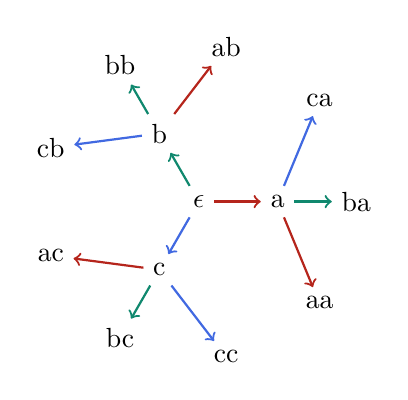
\begin{tikzpicture}
        \node (e) at (0,0) {$\epsilon$};
        \node (a) at (0:1) {a};
        \node (b) at (120:1) {b};
        \node (c) at (240:1) {c};
        \node (aa) at (-40:2) {aa};
        \node (ba) at (0:2) {ba};
        \node (ca) at (40:2) {ca};
        \node (ab) at (80:2) {ab};
        \node (bb) at (120:2) {bb};
        \node (cb) at (160:2) {cb};
        \node (ac) at (200:2) {ac};
        \node (bc) at (240:2) {bc};
        \node (cc) at (280:2) {cc};
    
        \draw[thick,->,BrickRed] (e) -- (a);
        \draw[thick,->,PineGreen] (e) -- (b);
        \draw[thick,->,RoyalBlue] (e) -- (c);
    
        \draw[thick,->,BrickRed] (a) -- (aa);
        \draw[thick,->,PineGreen] (a) -- (ba);
        \draw[thick,->,RoyalBlue] (a) -- (ca);
    
        \draw[thick,->,BrickRed] (b) -- (ab);
        \draw[thick,->,PineGreen] (b) -- (bb);
        \draw[thick,->,RoyalBlue] (b) -- (cb);
    
        \draw[thick,->,BrickRed] (c) -- (ac);
        \draw[thick,->,PineGreen] (c) -- (bc);
        \draw[thick,->,RoyalBlue] (c) -- (cc);
    \end{tikzpicture}
\end{center}
We are in a sense building up new words from old words, 
a form of induction where we have some bases case (the empty word)
and three inductive operators: prepend \code{a}, prepend \code{b}, or 
prepend \code{c}.
Notice because we only pre-pend there is no ambiguity 
in this grammar, that is, $abc$ can only mean $a(bc)$.
% Similar to the natural numbers, strings are the type 
% of another algebra, a \emph{free monoid} it will be called.
% This will become the start of a future algebra is another algebra, with one nullary operator 
% $\epsilon$ and three unary operators {\color{BrickRed}a$\Box$}, 
% {\color{PineGreen}b$\Box$}, and {\color{RoyalBlue}c$\Box$}
% being the production rules, that is the tree colors of arrows.

We can again make this computational.
\begin{Fcode}[]
data String_abc = nil
            | 'a' s:String_abc
            | 'b' s:String_abc
            | 'c' s:String_abc
\end{Fcode}
\begin{Pcode}[]
class StringABC
  case Nil extends StringABC
  case A(tail:String) extends StringABC
  case B(tail:String) extends StringABC
  case C(tail:String) extends StringABC
sealed
\end{Pcode}
    
\index{\code{<<Accept>>}}\index{grammar!accepted}
This all gets a bit tedious as we can see there is a pattern of
\code{<Character> <String>}.  So we remedy this by first we fix an alphabet
separately as its own inductive grammar and make strings that use a variable alphabet.
We need one further adaptation, since we add in new production rules in 
the services our of our main one we now indicated the productions 
that are ultimately acceptable by \code{<<Accept>>}.
\begin{Gcode}[]
<Char> ::= a | b | c | d | e
<<String>> ::= 
           | <Char> <String>
\end{Gcode}
Translated to popular coding styles this might be:
\begin{Fcode}[]
data AB = a | b
data ABC = a | b | c 
data String Char = Empty 
            | Prepend( head:Char, tail:String) 
a2 = a:String AB
a3 = a:String ABC --- a different 'a'
\end{Fcode}
We read \code{String} and now taking a parameter \code{Char}
which we could be any alphabet, but here it is given the 
choice of [a,b] and [a,b,c].
Writing \lstinline{head:Char} or \lstinline{tail:String} 
indicates that head must come from the alphabet we chose 
and tail must be some already produced string, possibly empty.
Some readers might relate to a different dialect of 
programming such as the following
\begin{Pcode}[]
class AB
  case A extends Char;  case B extends Char;
sealed
class ABC
  case A extends Char;  case B extends Char;
  case C extends Char
sealed
class String[Char]
  case Empty extends String
  case Prepend( head:Char, tail:String) extends String
sealed
a2 = new Prepend[AB](a, Empty())
a3 = new Prepend[ABC](a, Empty())
\end{Pcode}
% \end{lstlisting}
Observe the similarities with Peano's natural numbers:
\begin{align}
     2 & \defeq S(S(0)) \tag{$\mathbb{N}$}\\
 \text{\lstinline{"me"}} & \defeq \text{\lstinline{Prepend('m',Prepend('e',Empty))}}
\tag{String}
\end{align}
The left-hand sides are merely notation for what the data really is on the right.
Both the successor and the \lstinline{Prepend} are operators that generate 
new values.  Later in you shall come to know these constructions as free algebras,
but they are also foundational to programming.



\subsection{Circular definitions}
In order to explain grammar we had to have strings, and now strings are 
explained by grammar.  This has the feeling of being circular or what 
is formally called \emph{impredicative} or \emph{meta}.   This in and of 
itself is not illegal but it is a place to be cautious.  Definitions that 
talk about themselves can often be engineered into paradoxes and contradictions.  In fact this is the nature of Russell's Paradox for set,
G\"odel's Incompleteness Theorems for Integers, and Turing's Halting problem 
for computation.  So is the theory of grammars going to lead to a contradiction?

There are many ways to secure ourselves in trusting some list of assumptions.
We could try to prove it is correct based on assumptions we already agree with.
That can be hard when you work with something so basic as a grammar which seems 
to be the starting point of writing down any mathematics.  That is, there is not much else we already agreed to here so what would we use to write about language if our problem is with the validity of language?

The second option to calm concerns of contradiction is to create an example 
that obeys the claims of the theory.  If there were a contradiction in the theory that would mean a contradiction lives also in the example.  So if the 
example is trusted then the theory ought to be as well.  In that spirit I put to you that you have the model for grammar already: you are reading this 
sentence.  So the concept of grammar is validated by our communication and 
no more evidence is required on my part.